\documentclass[10pt,twocolumn]{article}
\usepackage[utf8]{inputenc}
\usepackage{amsmath}
\usepackage{amsfonts}
\usepackage{amssymb}
\usepackage{graphicx}\usepackage[left=1in,right=1in,top=1in,bottom=1in]{geometry}
\graphicspath{{img/}}

\title{\textbf{COMP90015 Project 2 \\ High Availability and Eventual Consistency\\}}

\author{\textbf{Thu Thao Le} (\texttt{thaol4@student.unimelb.edu.au})
\\[2ex] \textbf{Yicong Li} (\texttt{yicongl2@student.unimelb.edu.au})}

\date{}
\begin{document}
\maketitle

\section{Introduction}
The goal of this project is to implement new server protocol to address the server failure issues. The server can provide availability and eventual consistency among the servers and clients when network partioning happens. \\

There are many challenges in this project. The hardest part is to rebuild the server protocol to handle the failures in the network. We have used tree protocol with some improvements. \\

The result:

\section{Server failure}
There are three properties in our distributed systems: Consistency, Availability and Network partitions tolerance. According to CAP theorem \cite{eric}, we can only achieve at most two out of three properties. Since there are failures in the servers and the connections, we can only achieve either consistency or availability. If we choose availability, we can always return the messages even it is not up-to-date data. If we choose consistency, we have to update the latest data before returning the messages to clients. That means we can delay the sending process until all data is up-to-date or just return error when we cannot update the data. \\

There are three kinds of failures can happen in the system:
\begin{itemize}
\item Server crashes suddenly
\item Client crashes suddenly
\item Network is temporarily broken, then it can eventually be fixed.
\end{itemize}

The major problem in this project is how can we maximize the availability and consistency when network fails. There are three steps to handle the failure of the system \cite{eric12}:
\begin{itemize}
\item Detect the beginning of the failure
\item Limit some operations: There will be a trade-off between the consistency and availability. In this project, we focus on the availability during the partitions.
\item Recover the network: After recorvering the failures, we can eventually reach the consistency. 
\end{itemize}

\section{Server topology}
We use the tree structure to implement the server protocol in this project. However, we have some improvements to handle the network partitions. We set the hierarchy of the tree as in a family. As seen in the Fig. \ref{topo}, server 1 is the root server, which has two children: server 2 and server 5. Server 3,4 and 6 are the grandchildren of server 1. If the servers have the same parent, they are sibling. For example, server 3 is the older sibling of server 4. 
 


%\begin{figure}[h!]
%\begin{center}
%\includegraphics[scale=0.4]{topo1}
%\caption{First example of tree structure}	
%\end{center}
%\end{figure}

\begin{figure}[h!]
\begin{center}
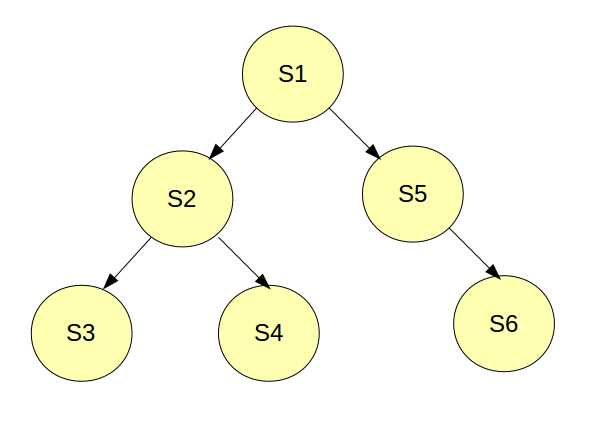
\includegraphics[scale=0.4]{full_topo}
\caption{Tree topology}
\label{topo}	
\end{center}
\end{figure}

\begin{figure}[h!]
\begin{center}
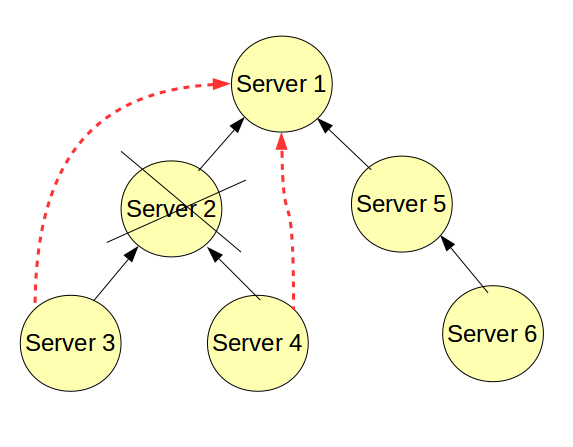
\includegraphics[scale=0.4]{parent_crash}
\caption{Parent server crashes, reconnect to root server}
\label{failroot}	
\end{center}
\end{figure}

\begin{figure}[h!]
\begin{center}
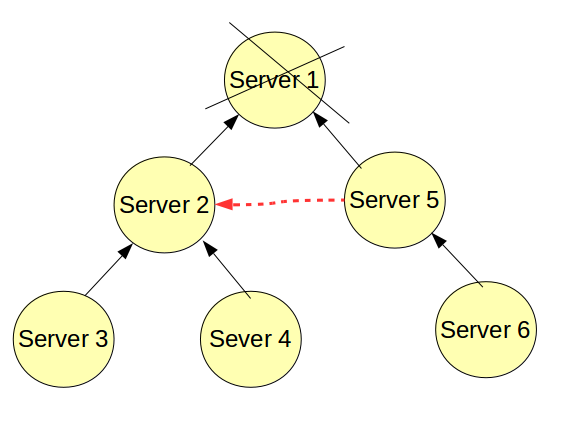
\includegraphics[scale=0.4]{root_crash}
\caption{Root server crashes, reconnect to the older sibling}
\label{failsibling}	
\end{center}
\end{figure}

Fig. \ref{failroot} and \ref{failsibling} describe two failure circumstances. In the first figure, server 2 crashes and then server 3 and 4 will connect to their grandparent, which is server 1. In the second situation as shown in Fig. \ref{failsibling}, root server crashes and server 2 and server 5 have no grandparent; therefore, the older sibling, which is server 2 will become the root server and server 5 will connect to its older sibling.

\begin{figure}[h!]
\begin{center}
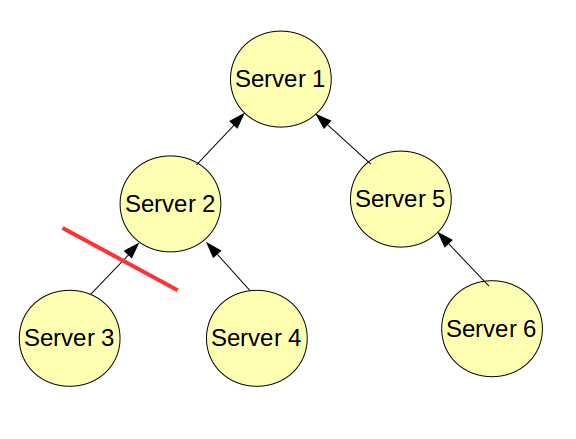
\includegraphics[scale=0.4]{network_broken}
\caption{Broken network between S2 and S3}
\label{broken}	
\end{center}
\end{figure}

Another failure that can happen is the broken network due to many reasons (E.g. turn off the wifi, etc). In this situation, we handle by following the process. 

As shown in Fig. \ref{broken}, there is no connection between server 2 and server 3.  We assumed that the network partitions is temporary and can eventually be fixed in less than 12 seconds. In this situation, server 3 will try to reconnect to server 2 in every 6 seconds. After two attempts of trying (exceeds 12s) and it still cannot connect to the server 2, server 3 will try to connect to its grandparent server, which is server 1. If server 2 does not have grandparent server, it will try to connect to its sibling server. If all attempts are failed, the connection of server 3 is closed and it will be removed out of the servers system.

\section{Implementation}
We implemented many functions in the server side to get the highest accuracy and consistency as possible, as well as an improvement of the first project. These functions will be described as follow. \\

The first improvement is that the servers can join the network after clients have joined. To fix this problem, we implemented a function to synchronize all user information from the remote server to the new server. The example below will illustrate this method.



	\subsection{Availability}

	\subsection{Eventual Consistency}

\section{Conclusion}

%\section{Demonstration}
%
%	\subsection{Server crashes}
%\begin{enumerate}
%\item Root server crashes, two children servers have to connect to each other (sibling connection).
%
%Root server (S1 -lp 3780 -rp 3780 -rh null -lh localhost) (CHECK!) \\
%Two children servers: (S2 -lp 3781 -rp 3780 -rh localhost), (S3 -lp 3782 -rp 3780 -rh localhost) 
%
%\item Parent server crashes, children servers connect to grandparent server.
%
%\end{enumerate}



\begin{thebibliography}{9}
\bibitem{eric} 
Eric Brewer
\textit{Towards robust distributed systems}. Jan, 2000.

\bibitem{eric12}
Eric Brewer
\textit{CAP Twelve Years Later: How the “Rules” Have Changed}. Feb, 2012.
\end{thebibliography}

\end{document}